\chapter{Articles Summary}{
	\label{chap:ArticleSummary}
	\section{A Co-Design Approach for Fault-Tolerant Loop Execution on Coarse-Grained Reconfigurable Arrays }{
		Article: \cite{FT_adaptive_loop_execution}
		
		Year: 2015
		
		This article create a hardware/software co-design configurable on reliability of application and on real time SER (Soft error rate). The techniques used are Coarse-Grained Reconfigurable Arrays (CGRAs), DMR and TMR.
	}
	\section{A dependence graph-based approach to the design of algorithm-based fault tolerant systems}{
		Article: \cite{ABFT_method_graph_based}
		
		Year: 1990		
		
		This article propose a two stage ABFT (Algorithm-based fault tolerance) system for computation intensive applications\cite{ABFT_method_graph_based} ABFT is a method invented in 1984 in this article "Algorithm-Based Fault Tolerance for Matrix Operations" \cite{ABFT_method}, the basic method encode data at high level and then the algorithm work on this data producing an encoded output. The computation is distributed along many unit to enhance fault tolerance, the method was first applied to matrix operation which are the basis of many intensive calculation. ABFT method can detect and correct errors in many matrix operation, to do this many processors are needed \cite{ABFT_method} . ABFT is a low cost CED (Concurrent error detection) scheme and fault location scheme \cite{ABFT_method_graph_based}.
		ABFT is applied to: Multiplication, triangularization, fft, sorting, mesh array and hypercubes (in a hypercube processor each processor is the corner of a cube and can communicate only with n other corner).
		This paper present a method to synthesize ABFT system based on graph-theoretic model and the use of dependence graph. The basic idea of the graph theoretic model is to use a checksum in the matrix for each processor, at the end of the computation the results are compared and a fault processor can be found. 
	}
	\section{A Methodology for Alleviating the Performance Degradation of TMR Solutions}{
		Article: \cite{Alleviate_TMR_preformance_degradation}
		
		Year: 2010
		
		Reliability degradation has increasing importance in faster and complex architecture due to sub 65nm technologies. In FPGAs the faults are more dangerous since can change design not just user data. TMR introduced by Xilinx ensures fault masking but increase chip area and power consumption, there is also a delay degradation due to redundancy that is catastrophic for critical application. This paper provide a method with reasonable balance between fault masking (F.M.) and performance/power overhead. Recent works use TMR in most sensitive subcircuits.   
		In this letter, we introduce a software supported frame-work that provides a trade-off between the desired level of fault masking and the performance/power degradation due to hardware redundancy. This is done by removing TMR from non sensitive subcircuits. The methods consist in the application of TMR to all processor, then the core is P\&R (Place and route) to FPGA and finally the temperature distribution is analyzed. Since temperature distribution give guidelines about where it is most likely faults to occur!! since the failure probability for a device region increases with temperature. So it is possible to eliminate redundancy from parts of the design that operate under low temperatures without affecting practically fault masking.Given the affordable level of errors for a design, our methodology guarantees to find the maximum redundancy that can be selectively removed from noncritical for failure regions of the device.
		\begin{figure}[H]
			\centering
			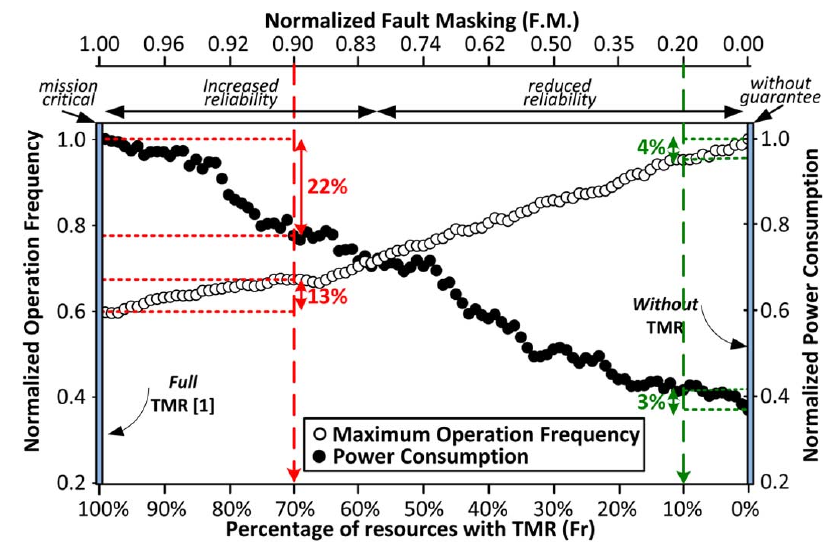
\includegraphics[scale=0.4]{./images/Articles_image/Alleviate_TMR_preformance_degradation_1.png}
			\caption{Different fault masking exploration}
			\label{Interface}
		\end{figure}
	}
	\section{An Analytical Approach for Soft Error Rate Estimation in Digital Circuits}{
		Article: \cite{SER_estimation_analytical}
		
		Year: 2005
		
		Soft error or transient errors also called SEU (Single event upset) are caused by particles. SER (Soft error rate) is the error rate due to SEUs, which depends both from particle flux both to circuit characteristic. Normally memory is more susceptible to errors, but from 2011 combinational logic will be comparable due to scaling. 
		This article propose the use of EPP (Error Propagation Probability) to estimate system failure due to soft errors. This method use the signal probability derived from power estimation calculus to derive a SER analytically. The complete algorithm is described. Final accuracy of 95\% and 4/5 times faster then fault injection techniques. 
	}
	\section{A new analytical approach to estimate the effects of SEUs in TMR architectures implemented through SRAM-based FPGAs}{
		Article: \cite{SEU_effect_in_TMR_analytical}	
		
		Year: 2005
		
		There are tree types of validation of an hardening techniques: 
		\begin{itemize}
			\item  accelerated radiation ground testing
			\item  Fault injection
		    \item  Analytical approach 
		\end{itemize}
		This paper propose and analytical approach. The main purpose of the proposed approach is to analyze the effects SEUs in both the user’s memory elements and the FPGAs configuration memory early in the design phase. 
	}
	\section{Automated design flow for applying Triple Modular Redundancy (TMR) in complex digital circuits}{
		Article: \cite{Automated_TMR_complex_digital_circuits}
		
		Year: 2018
		
		The main problem is that generation of FT redundancy is not supported by EDA tools. There are some tools such as Xilinx TMRTool, Synopsys Synplify Premier, and Mentor Precision HiRel were launched in the market to apply TMR during the synthesis process.
		This article  proposes an approach to automate the implementation, optimization, and verification of TMR circuits in commercial technologies. Three steps are added to the front-end design of ASICs. First, employing a post-synthesis netlist and according to the desired granularity level the TMR technique is applied, three different TMR versions of the circuit can be implemented automatically. Afterwards, gate sizing is performed over the resulting circuit in order to improve performance. Third, equivalence checking is used to verify both correct functionality and fault-tolerant capability of the TMR circuit with regards to the original circuit.
		TMR is implemented using Cadence’s synthesis tool Genus. The verification of FT architecture is done using Cadence’s Logic Equivalence Checking (LEC). Finally  simulation-based fault injections are performed to validate the effectiveness of the TMR implementation. 
	}
	\section{A voterless strategy for defect-tolerant nano-architectures}{
		Article: \cite{Voterless_defect_tolerance}
		
		Year: 2008
		
		This article explain how to use a reliable interconnect grid to create a voter for NMR hardening technique. It is an analog method!!
		The new communication mechanism is called LCDMA (Logic Code Division Multiple Access) and is implemented using an analog grid. Each signal that should be sent in the grid has to pass through a transmitter, the final signal should be analyzed to a receiver.
	}
	\section{Combining Correction of Delay Faults and Transient Faults}{
		Article: \cite{Combining_DelayF_and_TransF}
		
		Year: 2015
		
		Delay fault are fault caused by an extra delay in high speed logic that create a fault like a Transient fault due to particle. This paper use previous works such as Razor and Bubble Razor architecture to create a combining approach that can correct both delay and transient faults.
	}
	\section{Combining Fault Tolerance and Self Repair in a Virtual TMR Scheme}{
		Article: \cite{Combining_FT_and_self_repairing_virtual_TMR}
		
		Year: 2013
		
		This paper proposes a hardening architecture that allows both transient and permanent errors to be corrected using backup blocks. At startup, test vectors are used to understand the blocks with permanent errors and replace them by scoring the broken ones. In figure \ref{fig:timesharingtmr} you can see the time-sharing TMR.
		\begin{figure}[H]
			\centering
			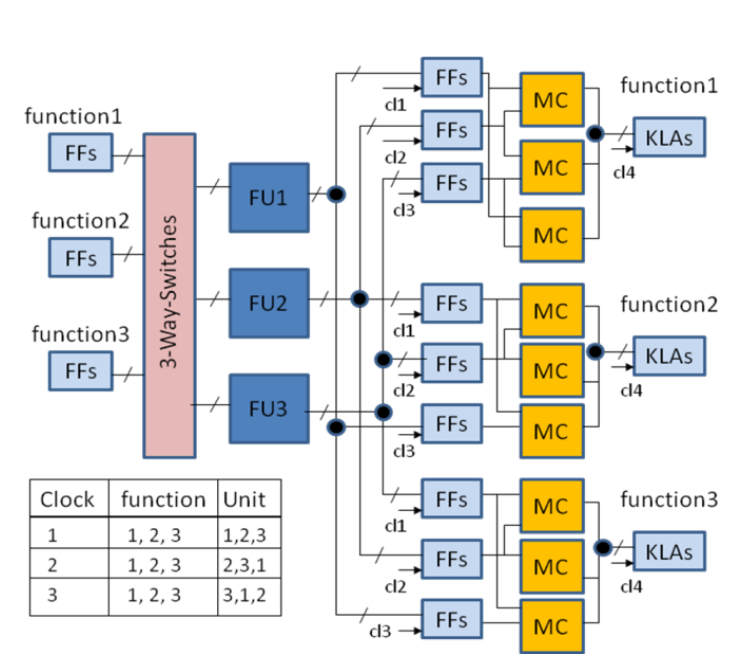
\includegraphics[scale=0.3]{./images/Articles_image/Combining_FT_and_self_repairing_ST_TMR.png}
			\caption{Time sharing TMR}
			\label{fig:timesharingtmr}
		\end{figure}	
		The extension of TS-TMR instead is in figure \ref{fig:timesharingtmr_selfrep}.
		\begin{figure}[H]
			\centering
			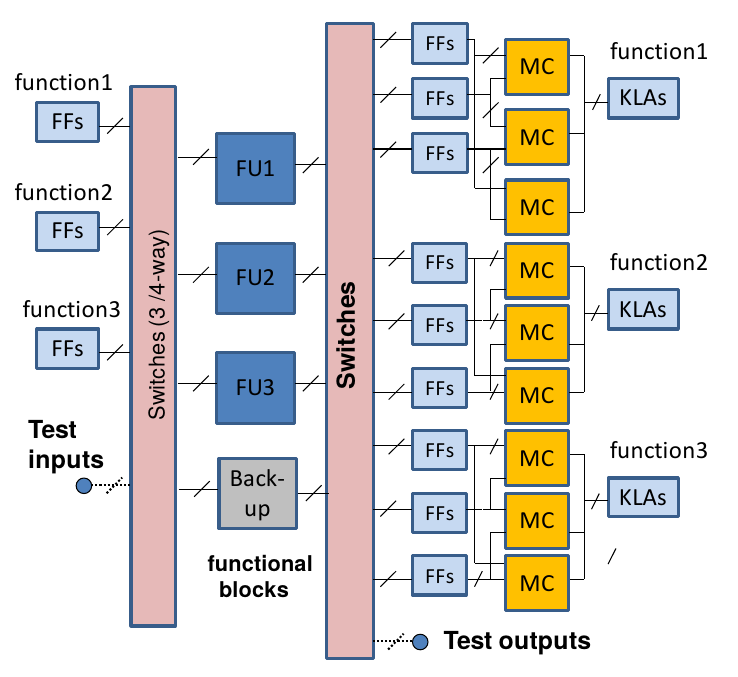
\includegraphics[scale=0.3]{./images/Articles_image/Combining_FT_and_self_repairing_ST_TMR_self_rep.png}
			\caption{Time sharing TMR}
			\label{fig:timesharingtmr_selfrep}
		\end{figure}
		In figure 	\ref{fig:timesharingtmr_Muller} you can see the Muller-C-element.
		\begin{figure}[H]
			\centering
			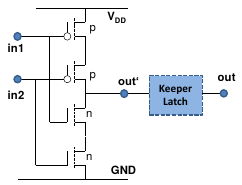
\includegraphics[scale=0.5]{./images/Articles_image/Combining_FT_and_self_repairing_Muller_C_element.png}
			\caption{Muller-C-element}
			\label{fig:timesharingtmr_Muller}
		\end{figure}	
		The proposed circuit has a 1/3 of the original throughput due to time sharing, the hardware is only one third of the original TMR. Also online self-repair is coupled with off-line self-repair.
	}
	\section{Error Detection and Fault Tolerance in ECSM Using Input Randomization}{
		Article:  \cite{Error_Detection_and_Fault_Tolerance_in_ECSM_Using_Input_Randomization}
		
		Year: 2009
		
		This paper discusses fault attacks on ECSM systems and proposes a technique based on parallel execution. This is similar to TMR but surpasses it by using the concepts of scaling and point randomization. This technique is more efficient and uses fewer blocks than TMR.
	}
	\section{Evaluating the effectiveness of a diversity TMR scheme under neutrons}{
		Article: \cite{Evaluating_the_effectiveness_of_a_diversity_TMR_scheme_under_neutrons}
		
		Year: 2013
		
		The paper evaluates the DTMR (Diversity Triple Modular Redundancy) using an FPGA hit by a neutron flux of \[3.98*10^4 n/cm^2/s\] (standard deviation of \[3.74*10^3 n/cm^2/s\]) with an energy of 10MeV for 1268 minutes. The average number of upsets detected was about one per minute. It was found that the DTMR approach is better than TMR because each redundant block has a different reliability. In figure  you can see the DTMR implementation used in the paper.
		\begin{figure}[H]
			\centering
			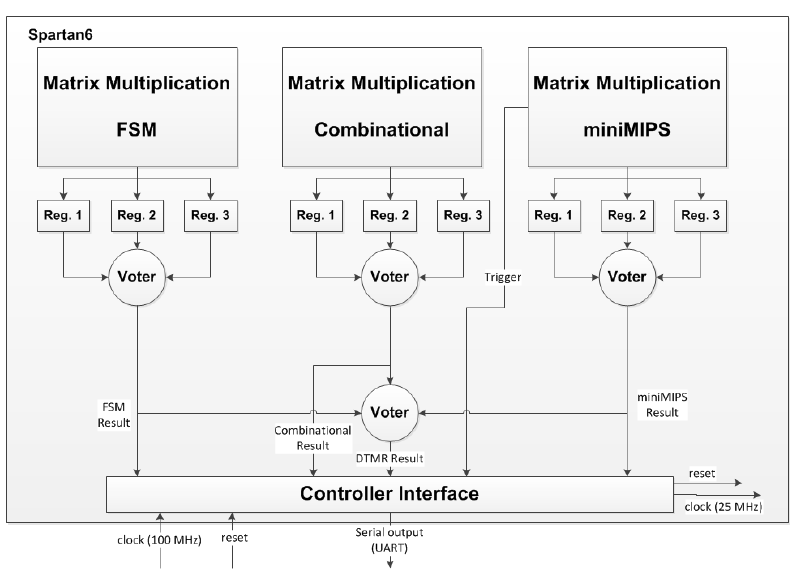
\includegraphics[scale=0.5]{./images/Articles_image/Evaluating_the_effectiveness_of_a_diversity_TMR_scheme_under_neutrons_DTMR.png}
			\caption{DTMR for matrix multiplication, tested using neutron beam}
			\label{fig:DTMR}
		\end{figure}			
	}
	\section{Fault and Soft Error Tolerant Delay-Locked Loop}{
		Article: \cite{Fault_and_Soft_Error_Tolerant_Delay-Locked_Loop}
		
		Year: 2020 
			
		The paper presents a new method to create fault tolerance DLLs based on the previous FET-DLL technique. The FET-DLL technique consisted in using three DLLs and voting the output clocks, the problem was in the delay due to the voter called "output-lagging". To solve this problem dummy voter are added in the feedback network of DLLs. Thanks to this technique you can have a fault tolerant DLL without delays.
		
	}
	\section{Hardware Error Correction using Local Syndromes}{
		Article: \cite{Hardware_error_correction_using_local_syndromes}
		
		Year: 2017	
		
		This article presents a method called DSC (Duplication with Syndrome based Correction) applicable only to signal processing domains where the operations belong to the homomorphisms group. This method is the evolution of TMR but with a 32\% simpler voter that allows an error correction very similar to that of TMR.
	}
	\section{Highly-Reliable Approximate Quadruple Modular Redundancy with Approximation-Aware Voting }{
		Article: \cite{Highly-Reliable_Approximate_Quadruple_Modular_Redundancy_with_Approximation-Aware_Voting}
		
		Year: 2020
		
		The paper proposes an approximate QMR redundancy method where are used three instances that approximate the true result and one that finds the exact one. A vote on the 3 approximate architectures is done first and then the result is voted with the exact architecture. The difference with the other works of approximate redundancy is in the use of approximators equal to each other while in the other works were used all different approximators.
	}
	\section{Low-Overhead Fault-Tolerance Technique for a Dynamically Reconfigurable Softcore Processor } {
		Article: molto lungo \cite{Low-overhead_fault-tolerance_technique_for_a_dynamically_reconfigurable_softcore_processor}
		
		Year: 2013
		
		The paper proposes a reconfigurable softcore processor for FPGAs that outperforms previous ones in terms of hardware and time costs reduction. A Configuration Engine is created to identify processor faults and once a fault is identified it can be removed by partial hardware reconfiguration or dynamic reconfiguration. This article use an Enhanced Lockstep Scheme.
	}
	\section{Low Overhead Soft Error Mitigation Techniques for High-Performance and Aggressive Designs}{
		Article: \cite{Low_Overhead_Soft_Error_Mitigation_Techniques_for_High-Performance_and_Aggressive_Designs}
		
		Year: 2012
		
		Two types of cells are proposed to mitigate soft errors. The first is called SEM cell \ref{fig:SEMCELL} \ref{fig:SEMCELLTIMING} and uses 3 clocks shifted between them to sample the input in 3 different registers . Register 1 is compared with register 2 to test an error, if there is an error the next block must recompute and the outputs of the other two registers are saved in register 1.
		The second cell is called STEM \ref{fig:STEMCELL} (Soft and timing error mitigation) is similar but more complex because it allows to restore a previous state and redo the computation.
		The advantage of this solution is that there is no overhead during normal error-free operations, but we need to redo computation.
		\begin{figure}[H]
			\centering
			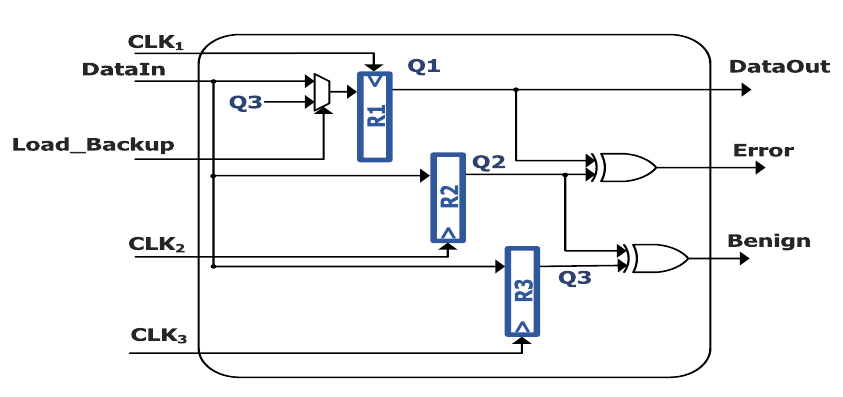
\includegraphics[scale=0.4]{./images/Articles_image/Low_Overhead_Soft_Error_Mitigation_Techniques_for_High-Performance_and_Aggressive_Designs_SEM.png}
			\caption{SEM cell}
			\label{fig:SEMCELL}
		\end{figure}
		\begin{figure}[H]
			\centering
			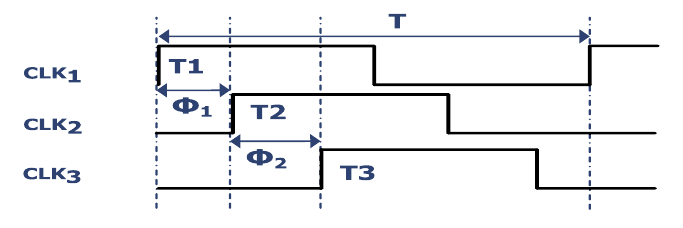
\includegraphics[scale=0.4]{./images/Articles_image/Low_Overhead_Soft_Error_Mitigation_Techniques_for_High-Performance_and_Aggressive_Designs_SEM_timing.png}  
			\caption{SEM cell timing}
			\label{fig:SEMCELLTIMING}
		\end{figure}
		\begin{figure}[H]
			\centering
			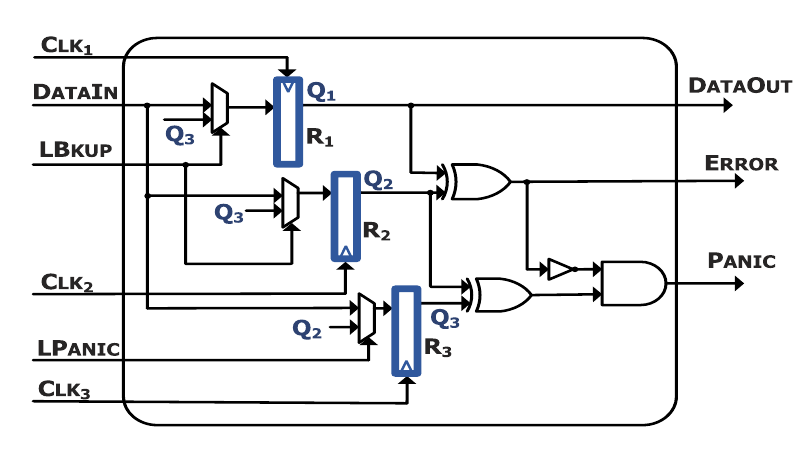
\includegraphics[scale=0.4]{./images/Articles_image/Low_Overhead_Soft_Error_Mitigation_Techniques_for_High-Performance_and_Aggressive_Designs_STEM.png}  
			\caption{STEM cell}
			\label{fig:STEMCELL}
		\end{figure}
	}
	\section{Optimization of a Cascading TMR System Configuration using Genetic Algorithm}{
		Article: \cite{Optimization_of_a_Cascading_TMR_system_configuration_using_Genetic_Algorithm}
		
		Year: 2012
		
		This paper uses a genetic algorithm to find the best TMR configuration, the triplication of blocks or/and voters is done in order to optimize area and relability. 
	}
	\section{Resilient Hardware Design for Critical Systems}{
		Article: \cite{Resilient_Hardware_Design_for_Critical_Systems}
		
		Year: 2019
		
		This paper proposes a structure formed by 3 redundant blocks and a different one that has the same function, the outputs are compared and an FSM evaluates which signal to give an output through a multiplexer. Calculations are made on the reliability of the system and it seems to be better than TMR.
	}
	\section{Scaling Analytical Models for Soft Error Rate Estimation Under a Multiple-Fault Environment}{
		Article: \cite{Scaling_Analytical_Models_for_Soft_Error_Rate_Estimation_Under_a_Multiple-Fault_Environment}
		
		Year: 2007
		
		The article starts from the analysis of Gurzi's method that allows to understand whether to use or not the TMR knowing the reliability of the voter and the circuit. Two methods are proposed to obtain the reliability of a circuit with TMR using the probability of the signals.
		
	}
	\section{Towards Byzantine fault tolerant publish/subscribe A state machine approach}{
		Article: \cite{Towards_Byzantine_fault_tolerant_publish_subscribe_A_state_machine_approach}
		
		Year: 2013
		
		The article discusses fault tolerance in the context of event-based interactions between systems. The BFT (Byzantine fault tolerance) pub/sub (publisher/subscriber) architecture based on an overlapping tree network is proposed.	
	}
}